\documentclass[11pt,a4paper]{article}
\usepackage[margin=2.6cm]{geometry}
\usepackage{amsmath,amssymb,amsthm}
\usepackage{graphicx}
\usepackage{booktabs}
\usepackage{microtype}
\usepackage[hidelinks]{hyperref}
\usepackage{xcolor}
\definecolor{ink}{HTML}{2430BC}
\hypersetup{colorlinks=true,linkcolor=ink,citecolor=ink,urlcolor=ink}
\usepackage[numbers,sort&compress]{natbib}


\newtheorem{proposition}{Proposition}
\theoremstyle{definition}
\newtheorem{definition}{Definition}
\theoremstyle{remark}
\newtheorem*{remark}{Remark}

\newcommand{\E}{\mathbb{E}}
\newcommand{\PP}{\mathbb{P}}
\newcommand{\avg}[1]{\langle #1 \rangle}

\graphicspath{{../figures/}}

\title{\textbf{When does a supply-chain failure reach the senior tranche?}\\[4pt]
\large Percolation thresholds and the distribution of structured credit losses}
\author{Kevin Grainger}
\date{October 2026}

\begin{document}
\maketitle

\begin{abstract}
\noindent
Structured credit models link defaults through a common economic factor. Firms are also linked directly, through supply chains, so that one failure can cause others. This note joins the two. It reviews the percolation theory of random networks, in which a failure spreads along each link with a fixed probability, and the threshold above which a single failure can reach a finite fraction of the network. It then derives the loss distribution of a portfolio whose obligors sit on such a network, and the expected loss of each tranche. Two results follow. First, with a single source of failure the probability that a tranche suffers any loss is discontinuous in the strength of contagion: it is zero until the giant failure cluster exceeds the attachment point, and then jumps. Second, in a calibrated model in which the economy sets the strength of contagion, matching the mean loss of a Vasicek model leaves the expected loss of the 15--30\% tranche about 46 times larger, while the equity tranche's falls by 40\%. Mean loss does not identify where in the capital structure the risk sits. Every analytic result is checked by Monte Carlo simulation on networks of $10^4$ firms. The percolation and cascade results are those of the cited authors; the application to tranche loss is the contribution of this note.
\end{abstract}

%=====================================================================
\section{Motivation: an ecologist's warning}
%=====================================================================

For most of the twentieth century ecologists held that complexity breeds stability: a food web with many species and many links between them should absorb shocks that would topple a simple one. In 1972 Robert May tested that belief with a short calculation and found it to be false \citep{May1972}. He took $N$ species, let a fraction $C$ of the possible pairs interact, and drew each interaction strength at random with standard deviation $\sigma$. Linearised about equilibrium, with each species self-regulating at unit rate, the community matrix has eigenvalues that, for large $N$, fill a disc of radius $\sigma\sqrt{NC}$ centred on $-1$. The system is stable almost surely when
\begin{equation}
\sigma\sqrt{NC} < 1 ,
\label{eq:may}
\end{equation}
and unstable almost surely when the inequality is reversed. Adding species, adding links or strengthening them all push a random system towards instability. The transition is sharp.

In 2008 the senior tranches of mortgage and corporate credit structures, rated as nearly riskless, lost value together. Writing in \textit{Nature} that year, May, Levin and Sugihara argued that bankers could learn from ecologists \citep{MayLevinSugihara2008}: risk had been assessed node by node, while the danger lay in the links. Haldane and May developed the argument with a model of interbank lending \citep{HaldaneMay2011}.

This note follows that thread to one precise question. A structured credit portfolio is usually priced as if its obligors default together only because they share an economy. Firms in a supply chain are also linked directly: a supplier that fails can take its customers with it. When does that direct linkage turn a local failure into a portfolio-wide one, and what does it do to the loss borne by each tranche?

%=====================================================================
\section{Percolation on random networks}
%=====================================================================

\subsection{The network}

Let $N$ firms be the nodes of a network. Firm $i$ has $k_i$ trading partners. The degrees are drawn independently from a distribution $p_k$, and partners are matched at random. This is the configuration model; for large $N$ it is locally tree-like, which is what makes the calculations below exact in the limit. Write $\avg{k} = \sum_k k p_k$ and $\avg{k^2} = \sum_k k^2 p_k$.

Following Newman, Strogatz and Watts \citep{NewmanStrogatzWatts2001}, the degree distribution is encoded in its probability generating function
\begin{equation}
G_0(x) = \sum_{k=0}^{\infty} p_k\, x^k .
\end{equation}
A firm reached by following a link is not a typical firm: it is $k$ times more likely to have degree $k$, because it has $k$ links by which to be reached. The number of its \emph{other} links, the excess degree, has generating function
\begin{equation}
G_1(x) = \frac{G_0'(x)}{G_0'(1)} = \frac{1}{\avg{k}} \sum_k k\, p_k\, x^{k-1}.
\end{equation}
Its mean is $G_1'(1) = (\avg{k^2} - \avg{k}) / \avg{k}$.

\subsection{Failure as bond percolation}

Suppose a failed firm causes each partner to fail independently with probability $T$, the \emph{transmissibility}. Equivalently, keep each link with probability $T$ and delete it otherwise; the firms that fail are those joined to a failed firm through kept links. This is bond percolation \citep{Callaway2000}.

Let $u$ be the probability that following a link from a firm does \emph{not} lead into the giant failure cluster, the cluster that occupies a finite fraction of the network. Either the link was deleted, with probability $1-T$, or it was kept and the firm at its far end is itself not connected to the giant cluster through any of its other links. On a tree those other links are independent, so
\begin{equation}
u = 1 - T + T\,G_1(u).
\label{eq:u}
\end{equation}
A random firm belongs to the giant cluster unless none of its links leads there, so the fraction of firms in it is
\begin{equation}
S = 1 - G_0(u).
\label{eq:S}
\end{equation}

\subsection{The threshold}

Equation \eqref{eq:u} always has the solution $u=1$, which gives $S=0$. A second solution with $u<1$ appears when the right-hand side crosses the diagonal at $u=1$ with slope greater than one, that is when $T\,G_1'(1) > 1$:
\begin{equation}
T > T_c = \frac{1}{G_1'(1)} = \frac{\avg{k}}{\avg{k^2} - \avg{k}} .
\label{eq:Tc}
\end{equation}
Below $T_c$ every failure stays local. Above it, a single failure reaches a fraction $S$ of all firms with probability $S$: the seed must itself lie in the giant cluster.

\paragraph{Poisson networks.} If partners are matched entirely at random, $p_k = e^{-c} c^k / k!$ with mean $c$, and $G_0(x) = G_1(x) = e^{c(x-1)}$. Then $T_c = 1/c$, and \eqref{eq:u}--\eqref{eq:S} reduce to
\begin{equation}
S = 1 - e^{-cTS}.
\end{equation}
Expanding for small $S$ gives $S \approx 2(cT-1)/(cT)^2$: the giant cluster grows linearly from zero above the threshold. Figure~\ref{fig:surface} shows $S$ over the plane of mean degree and transmissibility. The cliff along the curve $cT = 1$ is the phase transition.

\paragraph{Hubs.} For a power-law degree distribution $p_k \propto k^{-\gamma}$ with $2 < \gamma < 3$, $\avg{k^2}$ grows without bound as the largest degree grows, and $T_c \to 0$ \citep{Callaway2000, Cohen2000}. A network with a few very connected suppliers has almost no protective threshold.

\begin{figure}[t]
\centering
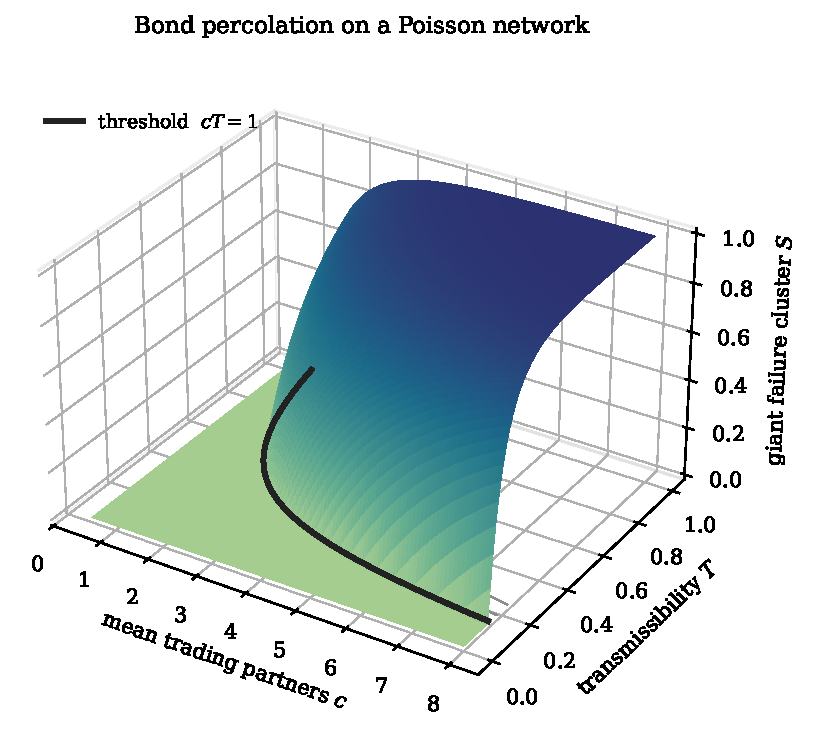
\includegraphics[width=0.78\textwidth]{fig1_percolation_surface.pdf}
\caption{Size $S$ of the giant failure cluster on a Poisson network, against mean number of trading partners $c$ and transmissibility $T$. Below the curve $cT=1$ every failure stays local.}
\label{fig:surface}
\end{figure}

\subsection{Below the threshold: amplification}

Below $T_c$ failures are finite, but not small near the threshold. The mean number of firms brought down by one failure, the seed included, is \citep{Newman2002}
\begin{equation}
\avg{s} = 1 + \frac{T\,G_0'(1)}{1 - T\,G_1'(1)} ,
\label{eq:amplification}
\end{equation}
which for a Poisson network is $1 + cT/(1-cT)$. It diverges at $T_c$. In the language of statistical physics this is the susceptibility; in the language of credit it is the factor by which supply-chain contagion multiplies own-cause defaults.

%=====================================================================
\section{Directed supply networks}
%=====================================================================

Supply relations have a direction. A supplier's failure halts its customers' production; a customer's failure costs its suppliers a receivable, which is a different and often smaller shock. Let firms have $j$ suppliers and $k$ customers with joint distribution $p_{jk}$, and let failure pass from supplier to customer with probability $T$. The same argument on the directed tree \citep{NewmanStrogatzWatts2001} gives a giant out-cluster, the set of firms reachable from a typical failure, when
\begin{equation}
T\,\frac{\avg{jk}}{\avg{k}} > 1 .
\end{equation}
The threshold depends on the correlation between a firm's number of suppliers and its number of customers. Firms that both buy from many and sell to many, the assemblers and distributors at the middle of a chain, lower it most. Acemoglu, Carvalho, Ozdaglar and Tahbaz-Salehi \citep{Acemoglu2012} reach a related conclusion for output rather than default: when a few sectors supply many others, sector-level shocks do not average out in the aggregate.

%=====================================================================
\section{Threshold cascades and the robust-yet-fragile network}
%=====================================================================

Percolation assumes each link transmits independently. A firm with many customers may survive the loss of one. Watts \citep{Watts2002} replaced the transmissibility with a threshold: a firm fails once at least a fraction $\phi$ of its partners have failed. A firm of degree $k$ is \emph{vulnerable} if a single failed partner suffices, that is if $k \le 1/\phi$. Let $\rho_k = 1$ for vulnerable degrees and $0$ otherwise. Repeating the branching argument on vulnerable firms alone, global cascades are possible when
\begin{equation}
\sum_k k(k-1)\,\rho_k\, p_k > \avg{k} .
\label{eq:watts}
\end{equation}
For a Poisson network the condition holds over a window of mean degree. At the lower edge the network is too sparse to carry a cascade. At the upper edge firms have so many partners that few are vulnerable. Near the upper edge cascades are rare, but when one starts it takes almost the whole network: the cascade size jumps discontinuously, unlike the continuous percolation transition. Gai and Kapadia \citep{GaiKapadia2010} found the same behaviour in a model of interbank exposures and described the system as robust yet fragile: more connections make contagion less likely and larger when it occurs. Figure~\ref{fig:sim}(b) reproduces the window.

%=====================================================================
\section{Tranche loss}
%=====================================================================

\subsection{Tranches}

A portfolio loses a fraction $L$ of its notional. A tranche with attachment point $a$ and detachment point $d$ absorbs losses between $a$ and $d$; the fraction of the tranche written down is
\begin{equation}
\psi_{a,d}(L) = \frac{\min\{\max(L-a, 0),\, d-a\}}{d-a},
\end{equation}
and its expected loss is $\mathrm{EL}(a,d) = \E[\psi_{a,d}(L)]$. Each defaulted firm loses a fixed fraction $\ell$ of its exposure (loss given default). The portfolio is the $N$ firms of the network, with equal exposures.

\subsection{The benchmark: Vasicek}

In Vasicek's one-factor model \citep{Vasicek2002} firm $i$ defaults when $\sqrt{\rho}\,Z + \sqrt{1-\rho}\,\varepsilon_i$ exceeds $\Phi^{-1}(1-p)$, where $Z$ is the state of the economy, $\varepsilon_i$ is firm-specific noise, both standard normal, and $p$ is the default probability. With $Z$ oriented so that large values are bad years, conditional on $Z$ the defaults are independent, and for large $N$ the loss converges to
\begin{equation}
L(Z) = \ell\, \Phi\!\left(\frac{\Phi^{-1}(p) + \sqrt{\rho}\, Z}{\sqrt{1-\rho}}\right).
\label{eq:vasicek}
\end{equation}
The default fraction $x = L/\ell$ has density
\begin{equation}
f(x) = \sqrt{\frac{1-\rho}{\rho}}\; \exp\!\left( \tfrac12 \Phi^{-1}(x)^2 - \frac{\big(\sqrt{1-\rho}\,\Phi^{-1}(x) - \Phi^{-1}(p)\big)^2}{2\rho} \right),
\end{equation}
single-humped with a tail that thins quickly. Firms are linked only through $Z$.

\subsection{A single source of failure: the loss is two-point}

Suppose first that own-cause failures are rare: their number in a year is Poisson with mean $\lambda$, independent of the network. In the large-$N$ limit each seed either lies in the giant cluster, with probability $S$, or sets off a finite cluster whose share of the portfolio vanishes. So
\begin{equation}
L \to \begin{cases} \ell S & \text{with probability } 1 - e^{-\lambda S}, \\ 0 & \text{otherwise.} \end{cases}
\end{equation}

\begin{proposition}
In this limit the expected loss of tranche $[a,d]$ is
\begin{equation}
\mathrm{EL}(a,d) = \big(1 - e^{-\lambda S}\big)\, \psi_{a,d}(\ell S),
\end{equation}
which is zero for $T \le T_c$. The probability that the tranche suffers any loss,
\begin{equation}
\PP(L > a) = \big(1 - e^{-\lambda S}\big)\, \mathbf{1}\{\ell S > a\},
\end{equation}
is discontinuous at the transmissibility $T_a > T_c$ at which $\ell S(T_a) = a$. It jumps from zero to $1 - e^{-\lambda a/\ell}$.
\end{proposition}

\begin{proof}
Both expressions follow from the two-point distribution. $S$ is continuous and increasing in $T$ above $T_c$, so $\ell S$ crosses $a$ at a single point $T_a$; below it $\psi_{a,d}(\ell S) = 0$ and the indicator is zero, above it both are positive. At $T_a$, $1 - e^{-\lambda S} = 1 - e^{-\lambda a/\ell} > 0$.
\end{proof}

The expected loss is continuous but has a kink at $T_a$; the probability of being touched jumps (Figure~\ref{fig:switch}). A model calibrated on years with $T < T_a$ reports a senior tranche that has never been touched, and is right to, until it is wrong all at once. Every tranche below $\ell S$ is wiped out together, which is why the curves in Figure~\ref{fig:switch} merge.

\begin{figure}[t]
\centering
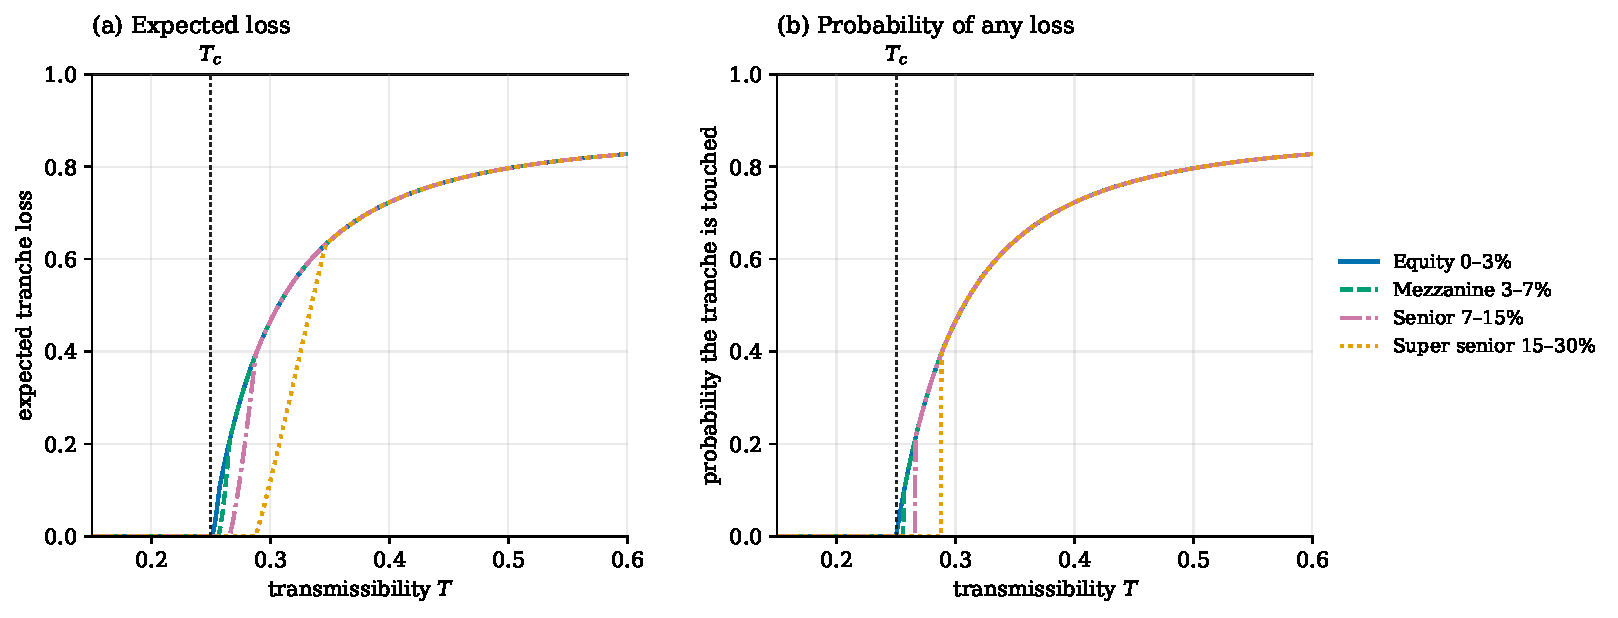
\includegraphics[width=\textwidth]{fig2_tranche_switch.pdf}
\caption{Single-seed model on a Poisson network with $c=4$ ($T_c = 0.25$), $\lambda = 2$ own-cause failures a year and loss given default $\ell = 0.6$. (a) Expected loss of each tranche. (b) Probability that each tranche suffers any loss: it jumps once the giant cluster passes the attachment point.}
\label{fig:switch}
\end{figure}

\subsection{Many sources of failure}

Own-cause defaults are not rare in a large portfolio: a fraction $p$ of firms fails each year regardless of the network. Let $v$ be the probability that a link, followed outward, does not transmit a failure back. Either it was deleted, or it was kept and the firm at the far end is not a seed and receives no failure through its other links:
\begin{equation}
v = 1 - T + T(1-p)\,G_1(v).
\label{eq:v}
\end{equation}
A firm survives if it is not a seed and no link brings it a failure, so the failed fraction is
\begin{equation}
F(p, T) = 1 - (1-p)\,G_0(v).
\label{eq:F}
\end{equation}
As $p \to 0$, $F$ tends to $S$ above $T_c$ and to $0$ below it; for small $p>0$ it rises steeply but smoothly through $T_c$, and below $T_c$ it is approximately $p\avg{s}$ from \eqref{eq:amplification}. Unlike the single-seed case, $F$ is deterministic: with a positive fraction of seeds the loss of a large portfolio no longer depends on where the first failure happened.

\subsection{The network-factor model}

The randomness must then come from somewhere else, and the natural place is the strength of contagion itself. In a good year a supplier's failure is absorbed: customers find other suppliers and banks extend credit. In a bad year the same failure spreads. Let the transmissibility depend on the state of the economy,
\begin{equation}
T(Z) = \Phi\!\left( \frac{\Phi^{-1}(\bar T) + \sqrt{\beta}\,Z}{\sqrt{1-\beta}} \right),
\end{equation}
so that $\bar T$ is its median and $\beta$ its sensitivity to the economy. The large-portfolio loss is
\begin{equation}
L(Z) = \ell\, F\big(p, T(Z)\big),
\label{eq:netfactor}
\end{equation}
which has the same structure as \eqref{eq:vasicek}: a deterministic function of one normal factor. In the Vasicek model the factor moves default probabilities; here it moves the network across its threshold. Tranche expected losses are one-dimensional integrals, $\mathrm{EL}(a,d) = \int \psi_{a,d}(L(z))\,\varphi(z)\,dz$, evaluated by quadrature.

\subsection{Equal mean, different tails}

Table~\ref{tab:cal} gives a calibration: a Poisson supply network with four partners per firm ($T_c = 0.25$), a 1\% own-cause default rate, a median transmissibility of 0.05 and $\beta = 0.4$. The network crosses its threshold in 3.8\% of years, about once in 26. The mean annual loss is 1.9\%. The Vasicek model is given the same mean loss and an asset correlation $\rho = 0.2$, within the range used for corporate portfolios.

\begin{table}[h]
\centering
\begin{tabular}{lll}
\toprule
Quantity & Symbol & Value \\
\midrule
Mean trading partners (Poisson) & $c$ & 4 \\
Own-cause default probability & $p$ & 1\% \\
Loss given default & $\ell$ & 60\% \\
Median transmissibility, sensitivity & $\bar T,\ \beta$ & 0.05,\ 0.4 \\
Probability the network is above threshold & $\PP(T(Z) > T_c)$ & 3.8\% \\
Mean annual loss (both models) & $\E L$ & 1.9\% \\
Vasicek asset correlation & $\rho$ & 0.2 \\
\bottomrule
\end{tabular}
\caption{Calibration of the network-factor model and its Vasicek comparison.}
\label{tab:cal}
\end{table}

\begin{table}[h]
\centering
\begin{tabular}{lrrrrr}
\toprule
Tranche & Network & Vasicek ($\rho=0.2$) & \multicolumn{3}{c}{Ratio, $\rho = 0.1,\ 0.2,\ 0.3$} \\
\midrule
Equity 0--3\% & 29\% & 47\% & 0.5 & 0.6 & 0.7 \\
Mezzanine 3--7\% & 4.5\% & 9.4\% & 0.8 & 0.5 & 0.4 \\
Senior 7--15\% & 3.4\% & 1.3\% & 17 & 2.7 & 1.3 \\
Super senior 15--30\% & 2.4\% & 0.052\% & 3{,}802 & 46 & 8.7 \\
Top 30--100\% & 0.31\% & 6.2e-05\% & $>10^4$ & 5{,}041 & 157 \\
\bottomrule
\end{tabular}

\caption{Expected tranche loss at equal mean portfolio loss. The last columns give the ratio for three Vasicek correlations.}
\label{tab:tranche}
\end{table}

The results are in Table~\ref{tab:tranche} and Figure~\ref{fig:equal}. At equal mean loss the network model gives the equity and mezzanine tranches \emph{less} expected loss than Vasicek, and the senior tranches far more: 2.7 times for the 7--15\% tranche and 46 times for the 15--30\% tranche. The reason is visible in the loss distribution. The network model puts most of its mass near the amplified own-cause loss $\ell p \avg{s}$, a little under 1\%, and the rest on a long, nearly flat plateau that reaches the size of the giant cluster. There is little in between. Risk moves up the capital structure. The ratio for the 15--30\% tranche ranges from 9 to several thousand as $\rho$ moves from $0.3$ to $0.1$; the direction does not change.

\begin{figure}[t]
\centering
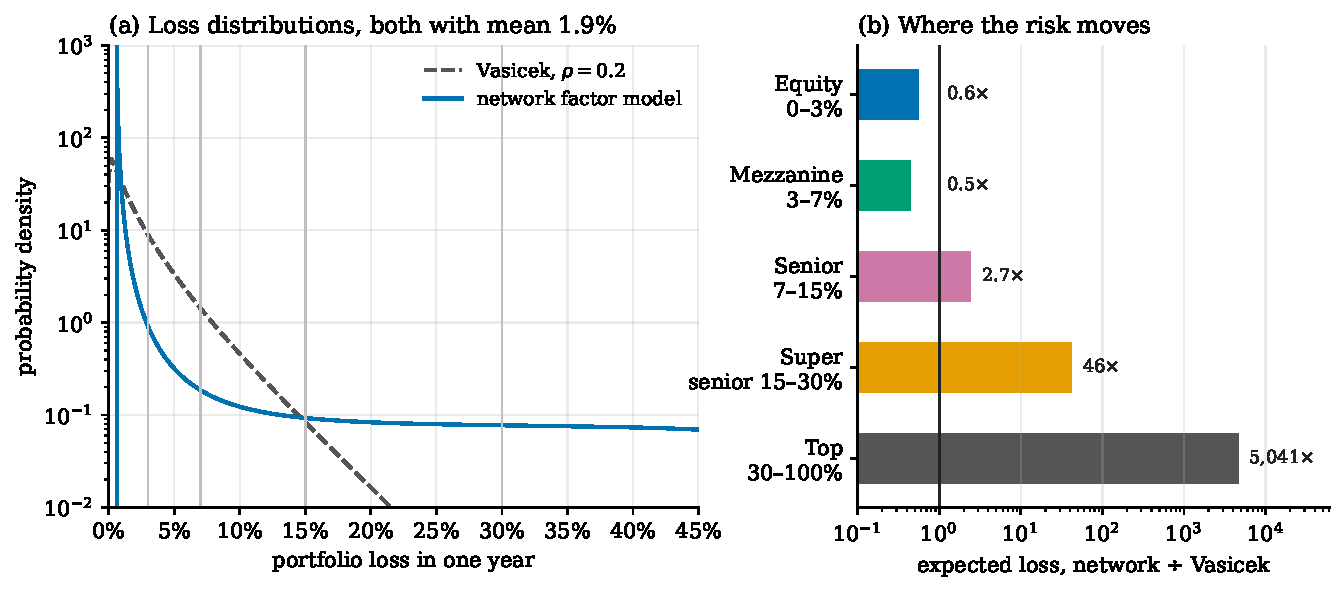
\includegraphics[width=\textwidth]{fig3_equal_mean.pdf}
\caption{Network-factor model against Vasicek at equal mean loss, calibration of Table~\ref{tab:cal}. (a) Loss densities; grey lines mark the tranche attachment points. (b) Ratio of expected tranche losses.}
\label{fig:equal}
\end{figure}

%=====================================================================
\section{Numerical check}
%=====================================================================

Each closed form above was checked by simulation on configuration-model networks of $N = 10^4$ firms, with self-loops and repeated links removed. For bond percolation, each link is kept with probability $T$ and the clusters found by a sparse connected-components search; Figure~\ref{fig:sim}(a) compares the largest cluster with $S$ from \eqref{eq:S} for a Poisson network and for a power law with $\gamma = 2.5$. Agreement is within the run-to-run spread away from the threshold; at the threshold the finite network rounds the transition, as expected. For the Watts model a single seed is failed and the cascade followed to completion, 400 times per mean degree; Figure~\ref{fig:sim}(b) shows the probability of a global cascade (more than 5\% of firms) and its size against the window predicted by \eqref{eq:watts}. The simulated window extends slightly past the analytic upper edge, where cascades remain possible on a finite network for a little longer; Watts reports the same \citep{Watts2002}. Near that edge the jump in cascade size is plain: at a mean degree of 6, 6\% of seeds set off a cascade, and each of those takes the entire network.

\begin{figure}[t]
\centering
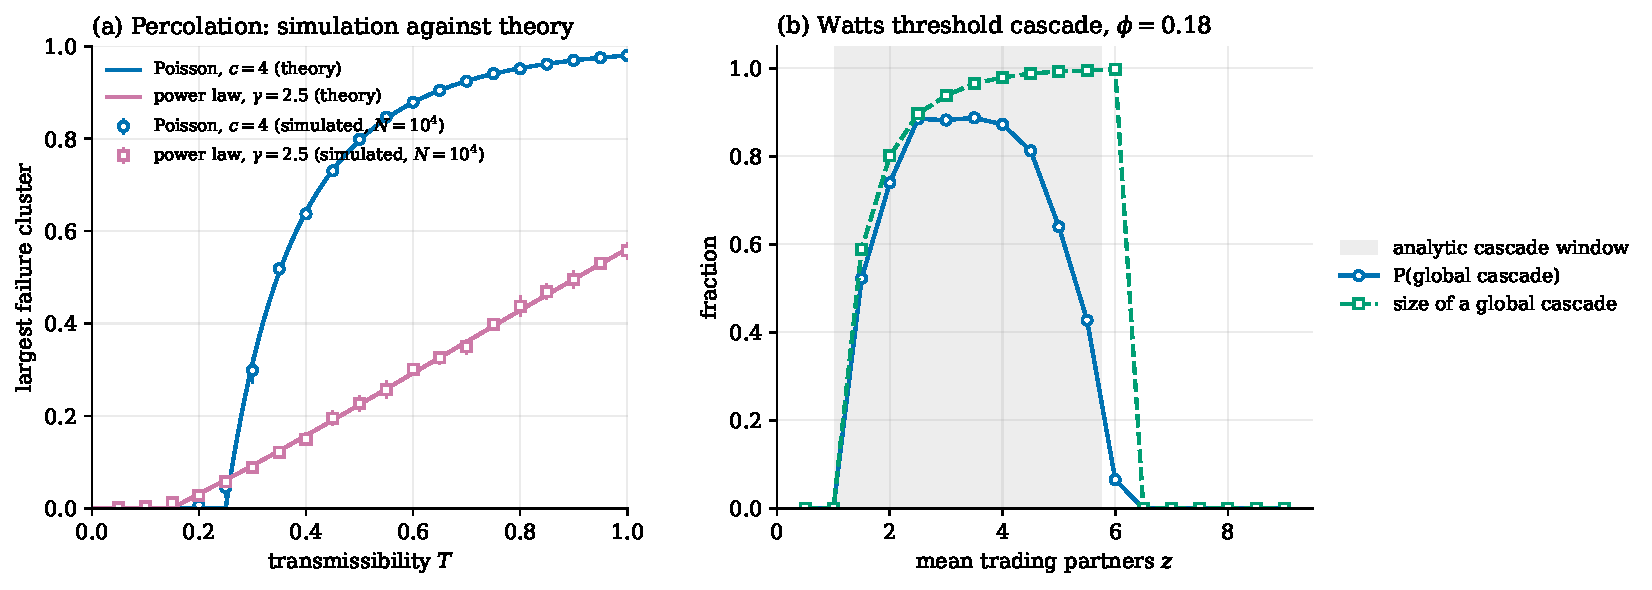
\includegraphics[width=\textwidth]{fig4_simulation_check.pdf}
\caption{(a) Largest failure cluster in simulation (markers, mean and standard deviation of 12 networks of $10^4$ firms) against theory (lines). (b) Watts threshold cascade with $\phi = 0.18$: probability and size of a global cascade, against the analytic window (shaded).}
\label{fig:sim}
\end{figure}

%=====================================================================
\section{Limits}
%=====================================================================

The network is random apart from its degree distribution. Real supply networks are clustered, assortative and geographically embedded, and percolation thresholds on such networks differ from \eqref{eq:Tc}. Links are static over the year; firms in fact replace failed suppliers, which lowers the effective $T$ with time. Loss given default is a constant, where in practice it is lower in bad years. Own-cause defaults are independent of the economy, where in practice they are not; a full model would let both $p$ and $T$ depend on $Z$. The portfolio is the whole network, where a real collateral pool holds a sample of it, and the giant cluster's overlap with a pool then matters. Nothing here is calibrated to a real portfolio: the calibration in Table~\ref{tab:cal} is chosen to give a plausible mean loss and frequency of crisis years. The result to take away is structural, not numerical: at fixed mean loss, contagion through a network with a threshold moves risk to the top of the capital structure.

%=====================================================================
\section*{Code}
%=====================================================================
All figures and tables are produced by \texttt{simulate.py}; the theory and simulation are in \texttt{percolation.py}.

\bibliographystyle{unsrtnat}
\begin{thebibliography}{99}
\bibitem[May(1972)]{May1972} R.~M. May. Will a large complex system be stable? \textit{Nature} 238, 413--414 (1972).
\bibitem[May et~al.(2008)]{MayLevinSugihara2008} R.~M. May, S.~A. Levin, G.~Sugihara. Ecology for bankers. \textit{Nature} 451, 893--895 (2008).
\bibitem[Haldane and May(2011)]{HaldaneMay2011} A.~G. Haldane, R.~M. May. Systemic risk in banking ecosystems. \textit{Nature} 469, 351--355 (2011).
\bibitem[Newman et~al.(2001)]{NewmanStrogatzWatts2001} M.~E.~J. Newman, S.~H. Strogatz, D.~J. Watts. Random graphs with arbitrary degree distributions and their applications. \textit{Phys. Rev. E} 64, 026118 (2001).
\bibitem[Callaway et~al.(2000)]{Callaway2000} D.~S. Callaway, M.~E.~J. Newman, S.~H. Strogatz, D.~J. Watts. Network robustness and fragility: percolation on random graphs. \textit{Phys. Rev. Lett.} 85, 5468--5471 (2000).
\bibitem[Cohen et~al.(2000)]{Cohen2000} R.~Cohen, K.~Erez, D.~ben-Avraham, S.~Havlin. Resilience of the Internet to random breakdowns. \textit{Phys. Rev. Lett.} 85, 4626--4628 (2000).
\bibitem[Newman(2002)]{Newman2002} M.~E.~J. Newman. Spread of epidemic disease on networks. \textit{Phys. Rev. E} 66, 016128 (2002).
\bibitem[Watts(2002)]{Watts2002} D.~J. Watts. A simple model of global cascades on random networks. \textit{Proc. Natl. Acad. Sci. USA} 99, 5766--5771 (2002).
\bibitem[Gai and Kapadia(2010)]{GaiKapadia2010} P.~Gai, S.~Kapadia. Contagion in financial networks. \textit{Proc. R. Soc. A} 466, 2401--2423 (2010).
\bibitem[Acemoglu et~al.(2012)]{Acemoglu2012} D.~Acemoglu, V.~M. Carvalho, A.~Ozdaglar, A.~Tahbaz-Salehi. The network origins of aggregate fluctuations. \textit{Econometrica} 80, 1977--2016 (2012).
\bibitem[Vasicek(2002)]{Vasicek2002} O.~Vasicek. The distribution of loan portfolio value. \textit{Risk} 15(12), 160--162 (2002).
\end{thebibliography}

\end{document}
